\documentclass[12pt,a4paper]{ctexart}
\usepackage{graphicx}
\usepackage{wrapfig}
\usepackage{float}
\usepackage{siunitx}
\usepackage{subfigure}
\usepackage{caption}
\usepackage{natbib}
\usepackage{listings} % 引入listings宏包用于插入代码
\usepackage{xcolor} % 引入xcolor宏包以支持更多的颜色设置

% 设置Verilog代码样式
\lstdefinestyle{verilog}{
    language=Verilog, % 设置语言为Verilog
    basicstyle=\small\ttfamily, % 设置基本字体样式
    keywordstyle=\color{blue}, % 关键字颜色设置
    commentstyle=\color{gray}\ttfamily, % 注释颜色和样式设置
    stringstyle=\color{red!60!black},
    numbers=left, % 行号在左边显示
    numberstyle=\tiny,
    frame=single, % 添加单线框
    rulecolor=\color{black!30}, % 边框颜色
    breaklines=true, % 允许自动换行
}

\title{实验 3:简单单周期 CPU}
\author{张子康 \ PB22020660}
\date{2024年04月15日}

\begin{document}
\maketitle
\newpage
\section{实验目的与内容}
\subsection{实验目的}
实现一个最为基础的单周期 CPU。
\subsection{实验内容}
\subsubsection{译码器设计}
根据自己选择的指令集,设计译码器 Decoder 模块,以正确生成控制信号。
\subsubsection{搭建 CPU}
正确实现 CPU 的各个功能模块,
并根据数据通路将其正确连接。
理论上,只需要完成 CPU 模块及其子模块的设计,而无需修改其他模块的内容。最终,你需要在 FPGAOL 上上板运行,并通过我们给出的测试程序,为此你需要实现 Lab1 列出的指令中,从 add.w(add)到 pcaddu12i(auipc)之间的全部指令。
\section{逻辑设计}
\subsection{译码器设计}
\begin{lstlisting}[style=verilog]
`define ADD                 5'B00000
`define SUB                 5'B00010
`define SLT                 5'B00100
`define SLTU                5'B00101
`define AND                 5'B01001
`define OR                  5'B01010
`define XOR                 5'B01011
`define SLL                 5'B01110
`define SRL                 5'B01111
`define SRA                 5'B10000
`define SRC0                5'B10001
`define SRC1                5'B10010
module DECODE (input [31 : 0] inst,
               output [4 : 0] alu_op,
               output [31 : 0] imm,
               output [4 : 0] rf_ra0,
               output [4 : 0] rf_ra1,
               output [4 : 0] rf_wa,
               output [0 : 0] rf_we,
               output [0 : 0] alu_src0_sel,
               output [0 : 0] alu_src1_sel);
reg [4:0] op;
reg [0:0] we;
reg [4:0] ra0;
reg [4:0] ra1;
reg [4:0] wa;
reg [0:0] src0_sel;
reg [0:0] src1_sel;
reg [31:0] imm_;

//初始化寄存器
initial begin
    op       = 0;
    we       = 0;
    ra0      = 0;
    ra1      = 0;
    wa       = 0;
    src0_sel = 0;
    src1_sel = 0;
    imm_     = 0;
end

assign alu_op       = op;
assign imm          = imm_;
assign rf_ra0       = ra0;
assign rf_ra1       = ra1;
assign rf_wa        = wa;
assign rf_we        = we;
assign alu_src0_sel = src0_sel;
assign alu_src1_sel = src1_sel;

always @(*) begin
    //R-type相关指令
    if (inst[6:0] == 7'b0110011) begin
        we       = 1;
        ra0      = inst[19:15];
        ra1      = inst[24:20];
        wa       = inst[11:7];
        src0_sel = 1'b0;
        src1_sel = 1'b0;
        imm_     = 32'h00000000;
        case ({inst[31:25], inst[14:12]})
            {7'b0000000, 3'b000}: op = `ADD;
            {7'b0100000, 3'b000}: op = `SUB;
            {7'b0000000, 3'b001}: op = `SLL;
            {7'b0000000, 3'b010}: op = `SLT;
            {7'b0000000, 3'b011}: op = `SLTU;
            {7'b0000000, 3'b100}: op = `XOR;
            {7'b0000000, 3'b101}: op = `SRL;
            {7'b0100000, 3'b101}: op = `SRA;
            {7'b0000000, 3'b110}: op = `OR;
            {7'b0000000, 3'b111}: op = `AND;
            default:              op = 5'b11111;
        endcase
    end
    //I-type相关指令
    else if (inst[6:0] == 7'b0010011) begin
        we       = 1;
        ra0      = inst[19:15];
        ra1      = 5'b00000;
        wa       = inst[11:7];
        src0_sel = 1'b0;
        src1_sel = 1'b1;
        imm_     = {{20{inst[31]}},inst[31:25]};
        case (inst[14:12])
            3'b000: op = `ADD;
            3'b010: op = `SLT;
            3'b011: op = `SLTU;
            3'b100: op = `XOR;
            3'b110: op = `OR;
            3'b111: op = `AND;
            3'b001: begin
                op   = `SLL;
                imm_ = {{27{inst[24]}},inst[24:20]};
            end
            3'b101:
            case (inst[31:25])
                7'b0000000:begin
                    op   = `SRL;
                    imm_ = {{27{inst[24]}},inst[24:20]};
                end
                7'b0100000:begin
                    op   = `SRA;
                    imm_ = {{27{inst[24]}},inst[24:20]};
                end
                default: op = 5'b11111;
            endcase
            default:op = 5'b11111;
        endcase
    end
    //U-type相关指令(lui)
    else if (inst[6:0] == 7'b0110111) begin
        we       = 1;
        ra0      = 5'b00000;
        ra1      = 5'b00000;
        wa       = inst[11:7];
        src0_sel = 1'b0;
        src1_sel = 1'b1;
        imm_     = {inst[31:12],12'b0};
        op       = `SRC1;
    end
    //U-type相关指令(auipc)
    else if (inst[6:0] == 7'b0010111) begin
            we       = 1;
            ra0      = 5'b00000;
            ra1      = 5'b00000;
            wa       = inst[11:7];
            src0_sel = 1'b1;
            src1_sel = 1'b1;
            imm_     = {inst[31:12],12'b0};
            op       = `ADD;
    end else begin
            we       = 0;
            ra0      = 5'b00000;
            ra1      = 5'b00000;
            wa       = 5'b00000;
            src0_sel = 1'b0;
            src1_sel = 1'b0;
            imm_     = 32'b0;
            op       = 5'b11111;
    end
end
endmodule
\end{lstlisting}
根据指令(inst),分别生成对应的
alu\underline{~}op,imm,rf\underline{~}ra0,
rf\underline{~}ra1,rf\underline{~}wa,
rf\underline{~}we,
alu\underline{~}src0\underline{~}sel,
alu\underline{~}src1\underline{~}sel。
\subsection{搭建 CPU}
\begin{lstlisting}[style=verilog]
`include "./include/config.v"

module CPU (
    input                   [ 0 : 0]            clk,
    input                   [ 0 : 0]            rst,

    input                   [ 0 : 0]            global_en,

/* ------------------------------ Memory (inst) ----------------------------- */
    output                  [31 : 0]            imem_raddr,
    input                   [31 : 0]            imem_rdata,

/* ------------------------------ Memory (data) ----------------------------- */
    input                   [31 : 0]            dmem_rdata, // Unused
    output                  [ 0 : 0]            dmem_we,    // Unused
    output                  [31 : 0]            dmem_addr,  // Unused
    output                  [31 : 0]            dmem_wdata, // Unused

/* ---------------------------------- Debug --------------------------------- */
    output                  [ 0 : 0]            commit,
    output                  [31 : 0]            commit_pc,
    output                  [31 : 0]            commit_inst,
    output                  [ 0 : 0]            commit_halt,
    output                  [ 0 : 0]            commit_reg_we,
    output                  [ 4 : 0]            commit_reg_wa,
    output                  [31 : 0]            commit_reg_wd,
    output                  [ 0 : 0]            commit_dmem_we,
    output                  [31 : 0]            commit_dmem_wa,
    output                  [31 : 0]            commit_dmem_wd,

    input                   [ 4 : 0]            debug_reg_ra,
    output                  [31 : 0]            debug_reg_rd
);


// TODO
wire [31:0] cur_npc;
wire [31:0] cur_pc;
wire [31:0] cur_inst;

//仿真时用于控制global_en信号,在上板时删除
assign global_en=!(cur_inst==32'H00100073);

//例化PC_PLUS4模块
PC_PLUS4 pc_plus(
.pc(cur_pc),
.pc_plus4(cur_npc)
);

//例化PC模块
PC pc(
.clk    (clk),
.rst    (rst),
.en     (global_en),   
.npc    (cur_npc),
.pc     (cur_pc)
);

//例化指令寄存器,从中读取指令
//可以不在cpu里例化,但实际没有影响
INST_MEM inst_mem(
//计算指令的位置
.a({{cur_pc-32'h00400000}/'d4}),    // input wire [8 : 0] a
.d(32'b0),      // input wire [31 : 0] d
.clk(clk),  // input wire clk
.we(1'b0),    // input wire we
.spo(cur_inst)  // output wire [31 : 0] spo
);

//定义decoder需要的变量
wire [4:0] rf_ra0;
wire [4:0] rf_ra1;
wire [4:0] rf_wa;
wire [31:0] rf_wd;
wire [4:0] alu_op;
wire alu_src0_sel;
wire alu_src1_sel;
wire [31:0] imm;
wire rf_we;
wire [31:0] rf_rd0;
wire [31:0] rf_rd1;

//例化decoder
DECODE decoder(
.inst(cur_inst),
.alu_op(alu_op),
.imm(imm),
.rf_ra0(rf_ra0),
.rf_ra1(rf_ra1),
.rf_wa(rf_wa),
.rf_we(rf_we),
.alu_src0_sel(alu_src0_sel),
.alu_src1_sel(alu_src1_sel)
);

//例化寄存器文件
REG_FILE reg_file(
.clk(clk),
.rf_ra0(rf_ra0),
.rf_ra1(rf_ra1),
.rf_wa(rf_wa),
.rf_we(rf_we),
.rf_wd(rf_wd),
.rf_rd0(rf_rd0),
.rf_rd1(rf_rd1),
.debug_reg_rd(debug_reg_rd),
.debug_reg_ra(debug_reg_ra)
);

//定义alu相关变量
wire [31:0] alu_src0;
wire [31:0] alu_src1;

//例化二选一数据选择器
MUX1 mux1(
    .src0(rf_rd0),
    .src1(cur_pc),
    .sel(alu_src0_sel),
    .res(alu_src0)
);
MUX1 mux2(
    .src0(rf_rd1),
    .src1(imm),
    .sel(alu_src1_sel),
    .res(alu_src1)
);

//例化alu
ALU alu(
    .alu_src0(alu_src0),
    .alu_src1(alu_src1),
    .alu_op(alu_op),
    .alu_res(rf_wd)
);

endmodule
\end{lstlisting}
在cpu中将所需的模块(算数逻辑单元(ALU)、寄存器堆(RF)、程序计数器(PC)、译码器(DECODER)、多路选择器(MUX)等。)
例化并连接到对应线路上。
\section{仿真结果与分析}
仿真时,向指令寄存器内导入制定的coe文件,仿真所用的
代码如下。
\begin{lstlisting}[style=verilog]
`timescale 1ns / 1ps
module tb_();
    reg clk;
    reg rst;
    wire [31:0] imem_raddr;
    wire dmem_we;
    wire [31 : 0]            dmem_addr;
    wire [31 : 0]            dmem_wdata;
    wire [ 0 : 0]            commit;
    wire [31 : 0]            commit_pc;
    wire [31 : 0]            commit_inst;
    wire [ 0 : 0]            commit_halt;
    wire [ 0 : 0]            commit_reg_we;
    wire [ 4 : 0]            commit_reg_wa;
    wire [31 : 0]            commit_reg_wd;
    wire [ 0 : 0]            commit_dmem_we;
    wire [31 : 0]            commit_dmem_wa;
    wire [31 : 0]            commit_dmem_wd;
    wire [31 : 0]            debug_reg_rd;
    //例化cpu模块并连接
    CPU cpu(
        .rst (rst),
        .clk (clk),
        .global_en(1'b1),
        .imem_rdata(0),
        .dmem_rdata(0),
        .debug_reg_ra(0),
        .imem_raddr(imem_raddr),
        .dmem_we(dmem_we),
        .dmem_addr(dmem_addr),
        .dmem_wdata(dmem_wdata),
        .commit(commit),
        .commit_pc(commit_pc),
        .commit_inst(commit_inst),
        .commit_halt(commit_halt),
        .commit_reg_we(commit_reg_we),
        .commit_reg_wa(commit_reg_wa),
        .commit_reg_wd(commit_reg_wd),
        .commit_dmem_we(commit_dmem_we),
        .commit_dmem_wa(commit_dmem_wa),
        .commit_dmem_wd(commit_dmem_wd),
        .debug_reg_rd(debug_reg_rd)
    );
    
    localparam CLK_PERIOD = 10;
    always #(CLK_PERIOD/2) clk=~clk;
    
    initial begin
        clk=0;
        rst=0;
        #10000
        $finish;
    end
    
endmodule
\end{lstlisting}
仿真结果如下:
\begin{figure}[H]
    \centering
    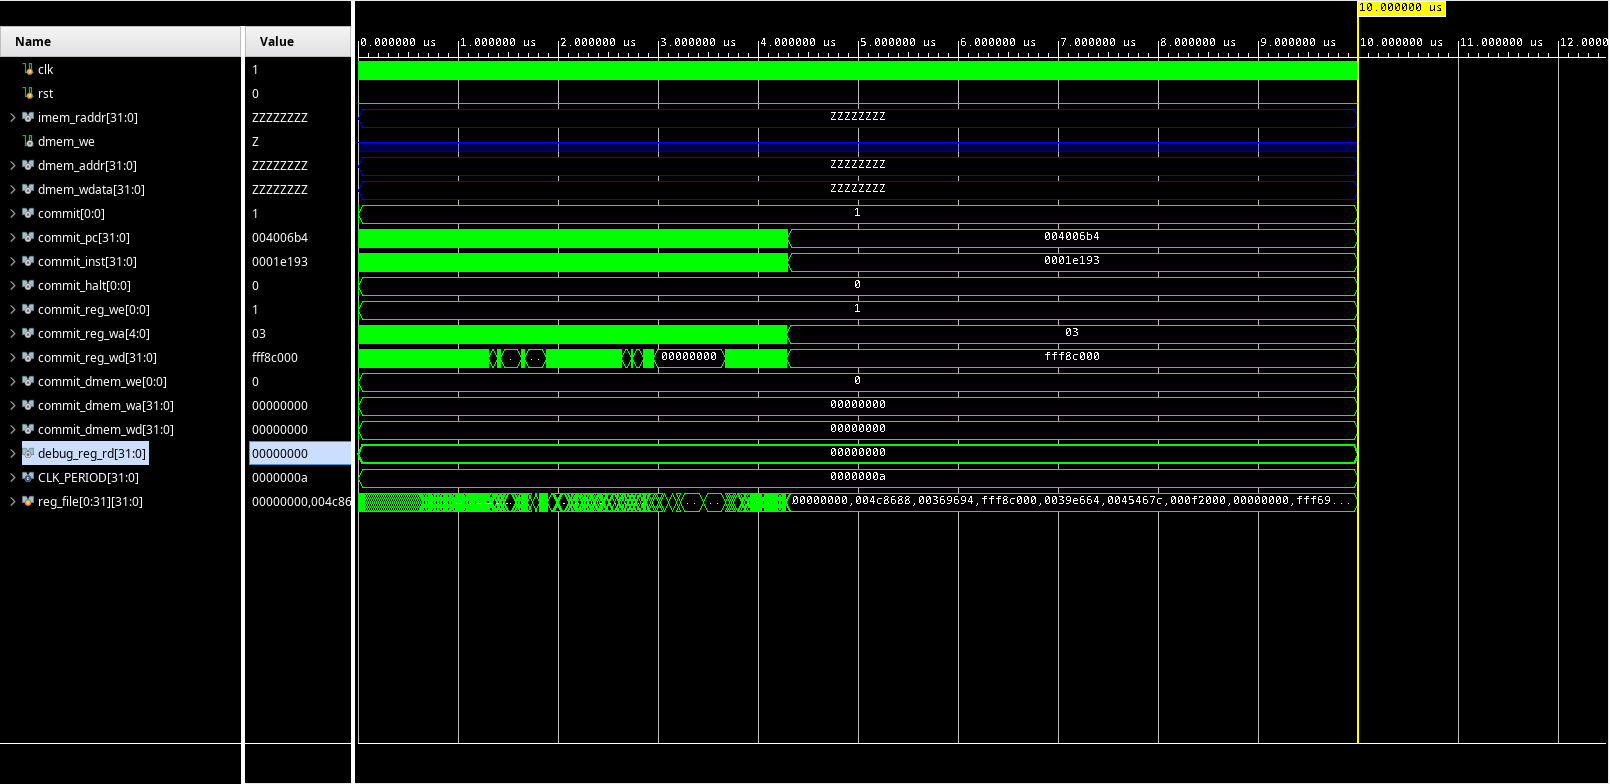
\includegraphics[scale=0.3]{pic/1.png}
    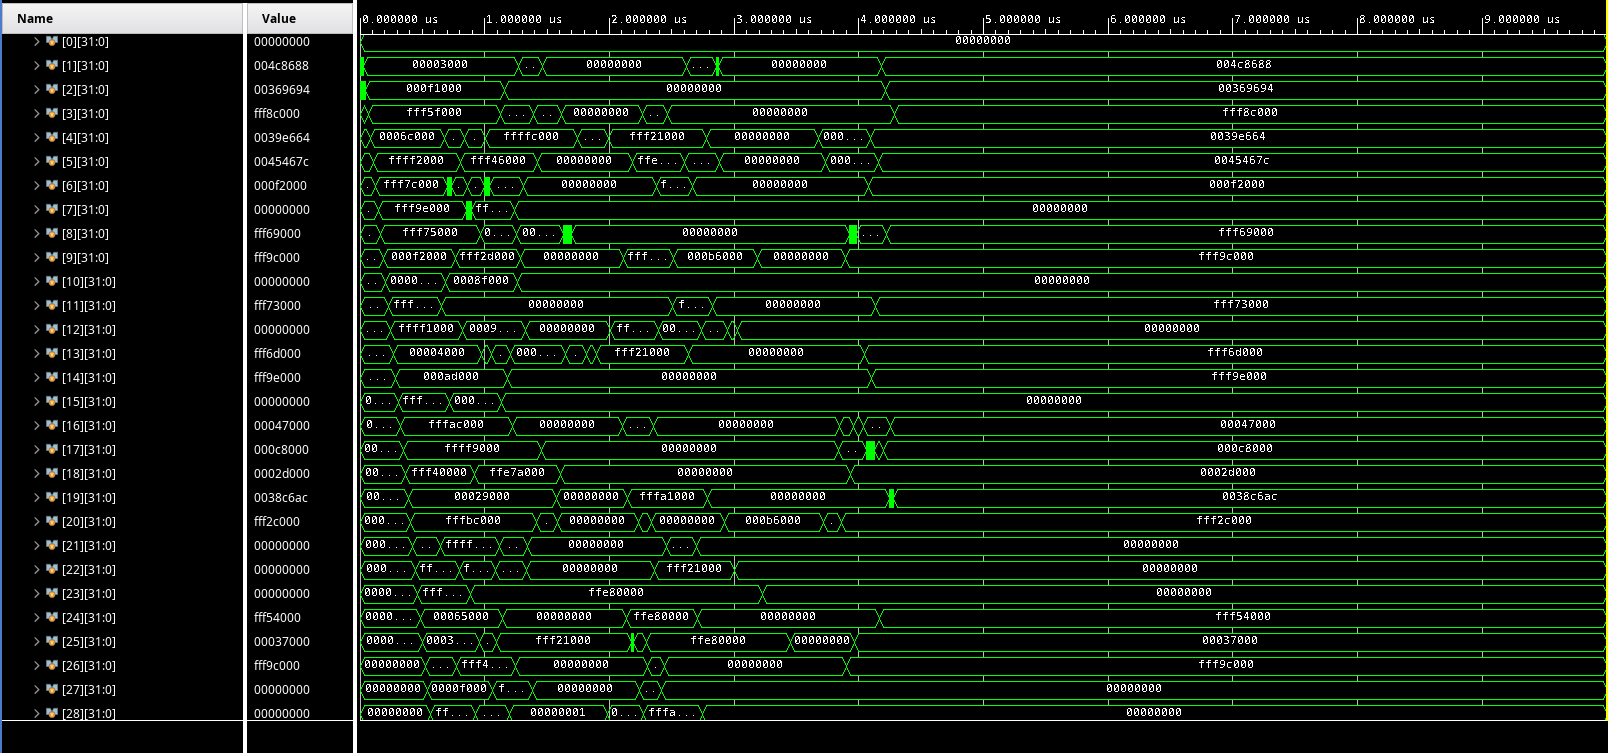
\includegraphics[scale=0.3]{pic/2.png}
    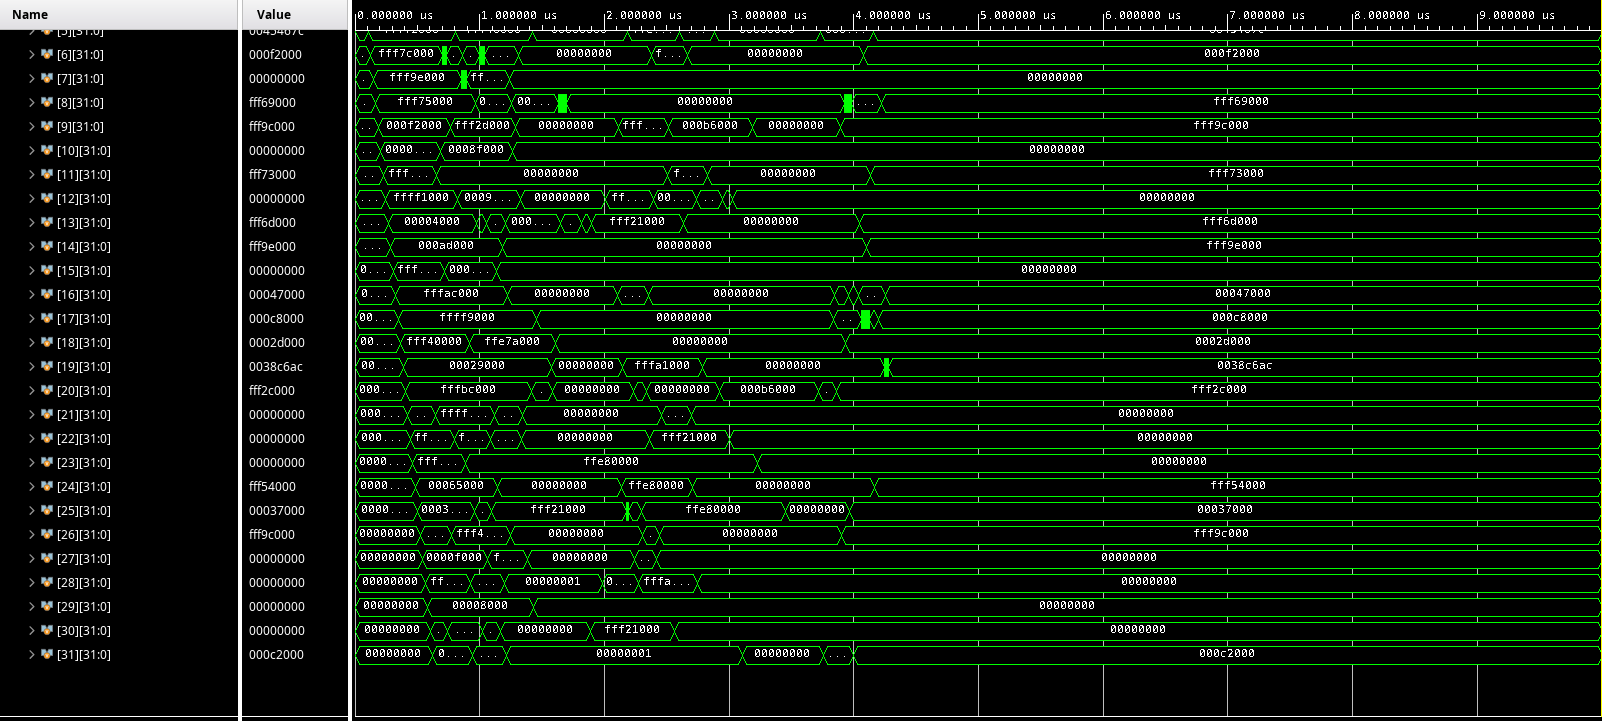
\includegraphics[scale=0.3]{pic/3.png}
    \caption{仿真结果}
\end{figure}
汇编程序运行结果如下:
\begin{figure}[H]
    \centering
    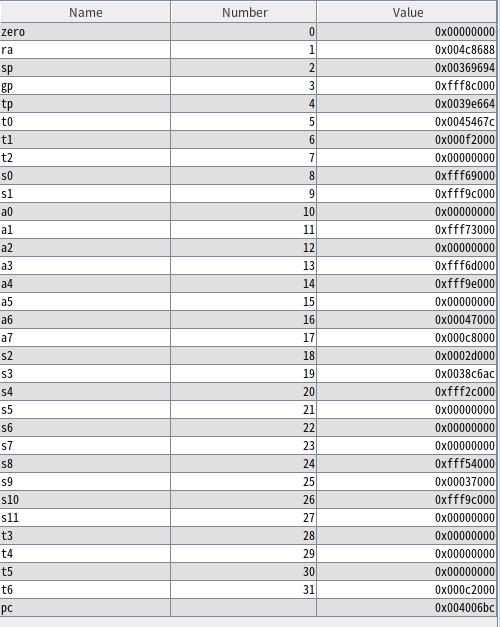
\includegraphics[scale=1]{pic/4.png}
    \caption{运行结果}
\end{figure}
证明了仿真结果的正确性。
\section{电路设计与分析}
cpu模块如图所示。
\begin{figure}[H]
    \centering
    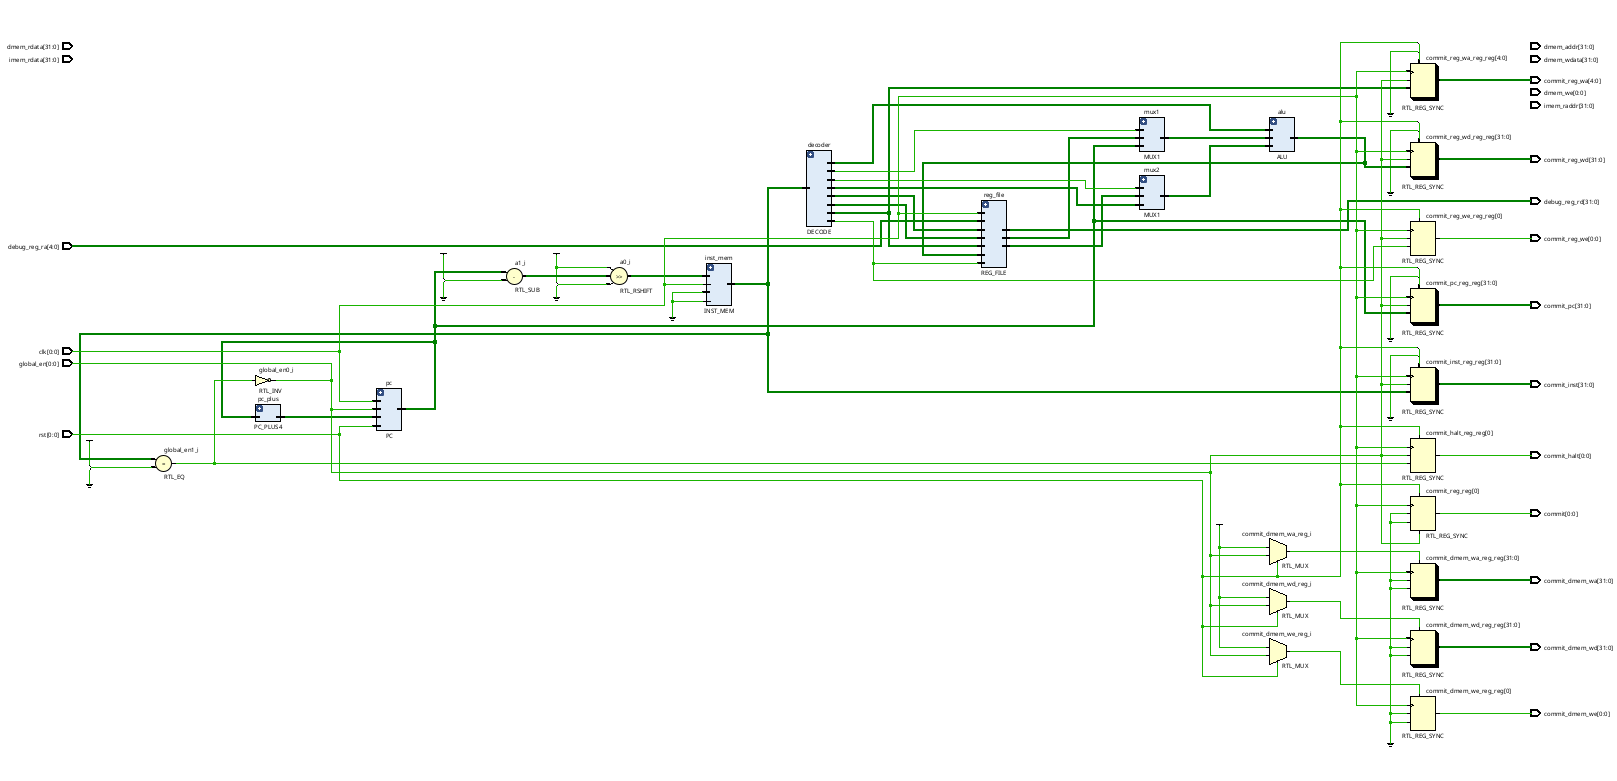
\includegraphics[scale=0.3]{pic/5.png}
    \caption{cpu模块}
\end{figure}
\section{测试结果与分析}
上板结果如下:
\begin{figure}[H]
    \centering
    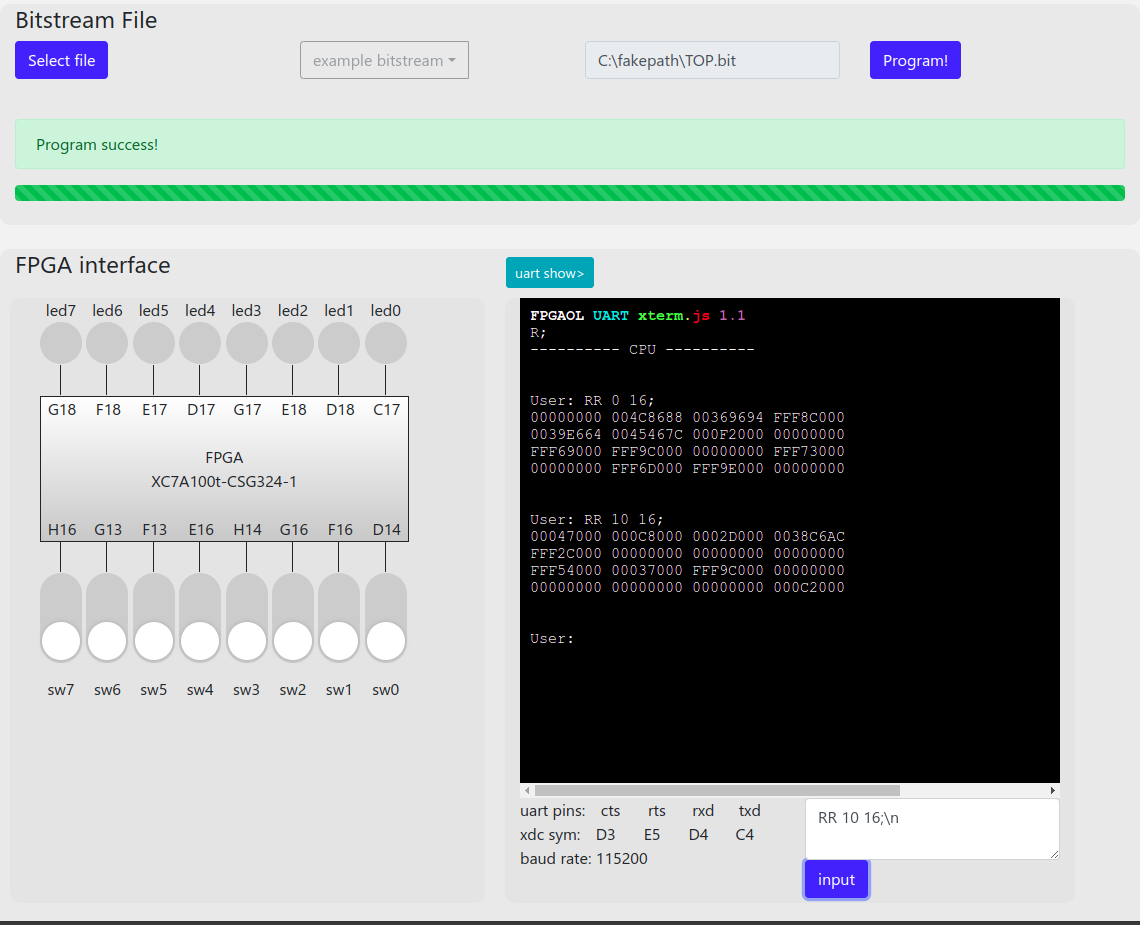
\includegraphics[scale=0.5]{pic/6.png}
    \caption{测试结果}
\end{figure}
结果与实际运行结果相吻合。
\section{思考与总结}
\subsection{本次实验的 CPU 中,哪些模块用到了时钟信号?}
PC模块,寄存器模块,指令存储器模块。
\subsection{请分别给出一条指令,以符合下面的描述:}
\subsubsection{alu\underline{~}src0 选择 pc}
auipc x17, 0xf2
\subsubsection{alu\underline{~}src0 选择 rf\underline{~}rd0}
addi x1,x1,1
\subsubsection{alu\underline{~}src1 选择 rf\underline{~}rd1}
add x1,x1,x2
\subsubsection{alu\underline{~}src1 选择 imm}
addi x1,x1,1
\subsection{请指出本次实验的 CPU 中可能的关键路径;如果这条路径的延迟大于一个时钟周期,可能会带来什么影响?}
\begin{figure}[H]
    \centering
    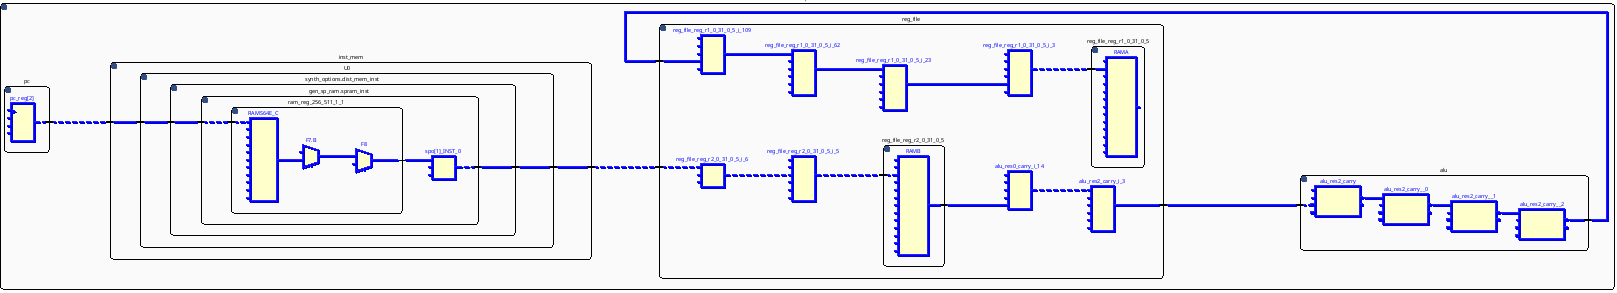
\includegraphics[scale=0.4]{pic/7.png}
    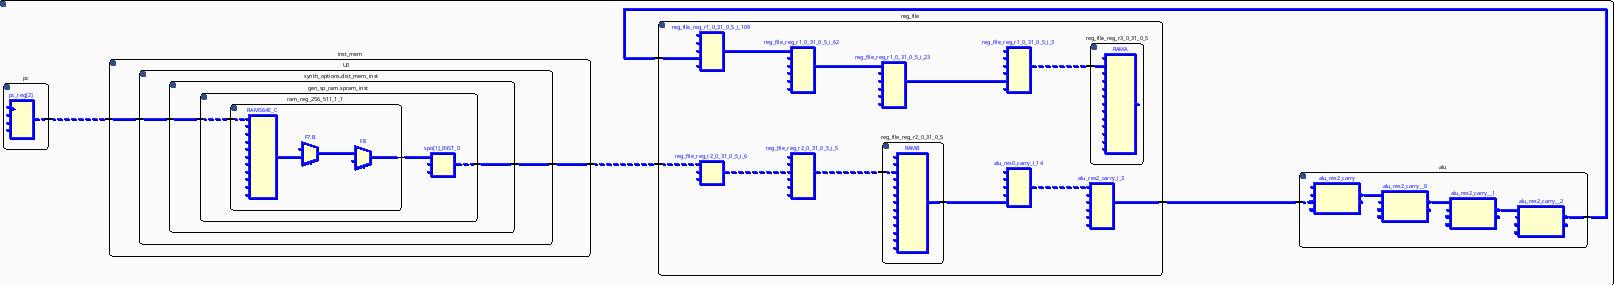
\includegraphics[scale=0.4]{pic/8.png}
    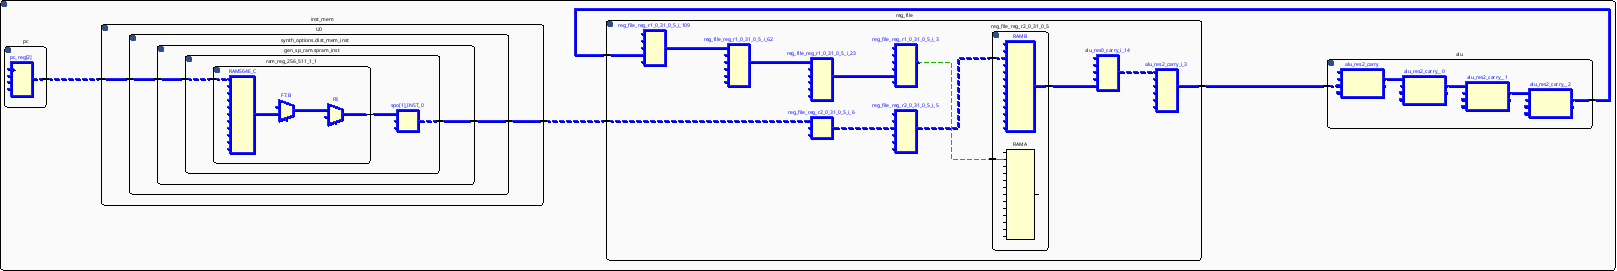
\includegraphics[scale=0.4]{pic/9.png}
    \caption{可能的关键路径}
\end{figure}
若这条路径的延迟大于一个时钟周期,
可能导致某些中间结果未能及时更新,
进而使得后续操作基于错误或过时的数据进行,
最终产生计算错误或指令执行失败。
\end{document}